% !TeX program = pdflatex
\documentclass[tikz,border=8pt]{standalone}
\usepackage{tikz}
\usetikzlibrary{calc,angles,quotes,positioning}
\definecolor{FigureBlue}{HTML}{2563EB}
\definecolor{FigureOrange}{HTML}{EA580C}
\definecolor{FigureGreen}{HTML}{16A34A}
\begin{document}
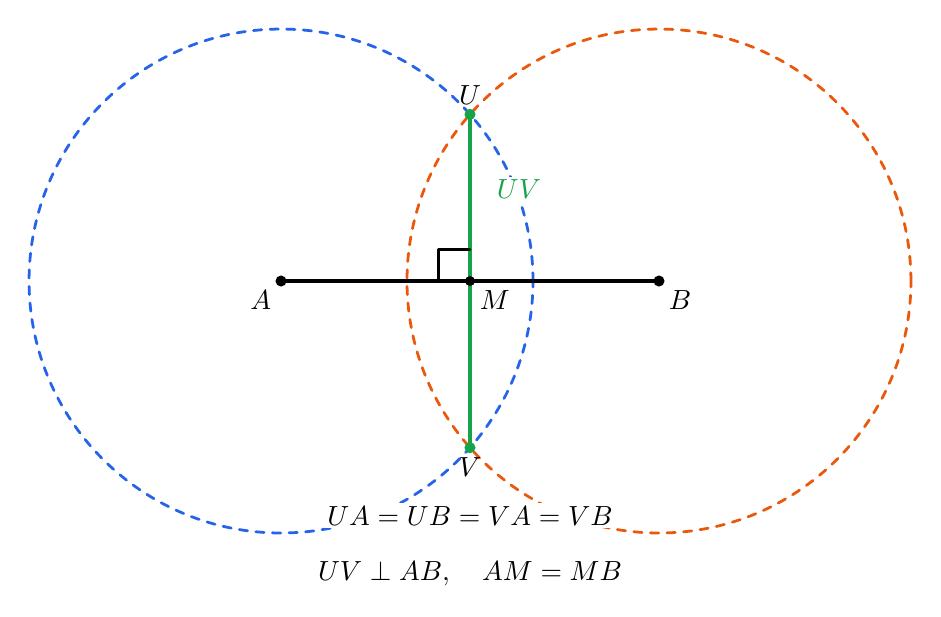
\begin{tikzpicture}[line cap=round,line join=round]
  \coordinate (A) at (-2.4,0);
  \coordinate (B) at (2.4,0);
  \coordinate (M) at ($(A)!.5!(B)$);
  \pgfmathsetmacro{\intersectionheight}{sqrt(3.2^2-2.4^2)}
  \coordinate (U) at (0,\intersectionheight);
  \coordinate (V) at (0,-\intersectionheight);

  \draw[FigureBlue,line width=1pt,dashed] (A) circle (3.2);
  \draw[FigureOrange,line width=1pt,dashed] (B) circle (3.2);
  \draw[line width=1.3pt] (A)--(B);
  \draw[FigureGreen,line width=1.6pt] (U)--(V);
  \pic[draw,line width=.9pt,angle radius=4mm] {right angle=A--M--U};

  \fill (A) circle (2pt) (B) circle (2pt) (M) circle (1.8pt);
  \fill[FigureGreen] (U) circle (2pt) (V) circle (2pt);
  \node[below left] at (A) {$A$};
  \node[below right] at (B) {$B$};
  \node[below right] at (M) {$M$};
  \node[above] at (U) {$U$};
  \node[below] at (V) {$V$};
  \node[right=3mm,FigureGreen,fill=white,inner sep=1pt] at ($(U)!.45!(M)$) {$UV$};
  \node[below=7mm of V,fill=white,inner sep=1pt] {$UA=UB=VA=VB$};
  \node[below=14mm of V,fill=white,inner sep=1pt] {$UV\perp AB,\quad AM=MB$};
\end{tikzpicture}
\end{document}
